\documentclass[a4paper]{article}

\usepackage[14pt]{extsizes} % чтобы использовать шрифт размером больше 12
\usepackage{cmap} % для кодировки шрифтов в pdf
\usepackage[T2A]{fontenc} % пакет указывает внутреннюю кодировку в системе LaTeX
\usepackage[utf8]{inputenc} % кодировка  
\usepackage[english, russian]{babel} % пакет для локализации

\usepackage{graphicx} % для вставки картинок
\usepackage{amssymb,amsfonts,amsmath,amsthm} % математические дополнения от АМС
\usepackage{indentfirst} % отделять первую строку раздела абзацным отступом тоже
\usepackage{makecell} % для создания таблиц
\usepackage{multirow} % для продвинутых таблиц
\usepackage{setspace} % для изменения междустрочного интервала
\usepackage{ulem} % подчеркивания

\usepackage[left=20mm, top=15mm, right=15mm, bottom=15mm, nohead, footskip=10mm]{geometry} % настройки полей документа

\linespread{1.3} % полуторный интервал
 
\begin{document} % начало документа
 
\section{Математическая постановка задачи}

Для решения общей задачи по нахождению деформаций и напряжений в деформируемом теле, занимающем область $G$ с границей $\partial \, G$, необходимо использовать следующие соотношения:

кинематические граничные условия
\begin{equation}
u(x) = u_0, \ x \in \partial \, G_D,
\end{equation}

силовые граничные условия
\begin{equation}
\sigma(u) \cdot n = p(x), \ x \in \partial \, G_N,
\end{equation}

соотношения Коши для тензора полных деформаций
\begin{equation}
\varepsilon(u)=\dfrac{1}{2}(\nabla u + (\nabla u)^T,
\end{equation}

тензор напряжений
\begin{equation}
\sigma(u)=???
\end{equation}

Здесь $u(x)$ - компоненты вектора перемещения, $\partial G_D$ - участок границы, на котором действуют кинематические условия Дирихле, $\partial G_N$ - участок границы, на котором действуют силовые граничные условия Неймана, $p(x)$ - вектор внешней нагрузки. 

Решить данную задачу можно с помощью метода декомпозиции Шварца.

\subsection{Методы Шварца}
Рассмотрим классическую задачу метода Шварца для двух подобластей: имеется сложная область $\Omega$, состоящая из объединения двух простых областей (круга $\Omega_1$ и прямоугольника $\Omega_2$). Рассмотрим уравнение Пуассона, цель которого найти перемещения $u: \Omega \rightarrow \mathbb{R}$ при условии, что
\begin{equation*}
\begin{array}{rl}
-\bigtriangleup \!(u) = f, & u \in \Omega \\
u = 0, & u \in \partial \Omega
\end{array}
\end{equation*}

\begin{figure}[h]
\center{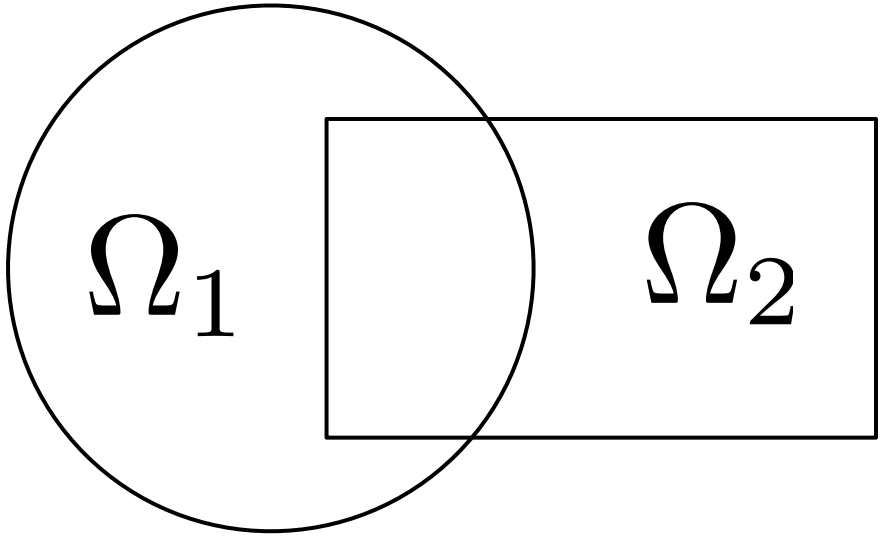
\includegraphics[scale=0.2]{img/simple_domains.png}}
\caption{Сложная область, получившаяся из объединения двух простых областей}
\label{fig:image_01}
\end{figure}

\newpage

Классический метод Шварца это итерационный метод, основанный на решении задач меньшего масштаба в подобластях $\Omega_1$ и $\Omega_2$. Один шаг итерационного процесса обновления результатов $u^n \rightarrow u^{n+1}$:
\begin{equation*}
\begin{array}{rl}
-\bigtriangleup \! (u^{n+1}) = f, & u \in \Omega_1 \\
u^{n+1} = 0, & u \in \partial \Omega_1 \cap \partial \Omega \\
u^{n+1} = u^n, & u \in \partial \Omega_1 \cap \bar{\Omega_2}
\end{array}
\textrm{после чего}
\begin{array}{rl}
-\bigtriangleup \! (u^{n+1}) = f, & u \in \Omega_2 \\
u^{n+1} = 0, & u \in \partial \Omega_2 \cap \partial \Omega \\
u^{n+1} = u^n, & u \in \partial \Omega_2 \cap \bar{\Omega_1}
\end{array}
\end{equation*}

Теперь же рассмотрим случай для произвольной области и произвольного числа подобластей. Вернёмся к нашей первоначальной задаче (ссылка здесь), представим область $G$ в виде объединения конечного числа подобластей $G = \bigcup_{i=1}^{M} G_i$ с конечным числом границ $\partial G_1, \ldots, \partial G_M$, где M - число подобластей. Данные подобласти пересекаются, что требует ввода дополнительных обозначений для границ, возникающих после декомпозиции областей: $\Gamma = \bigcup_{i=1}^{M} \Gamma_i$. 

Выберем начальное приближение для перемещений, удовлетворяющее граничным условиям (ссылка здесь). Алгоритм из классического метода Шварца можно оптимизировать для большего числа подобластей:
\begin{equation*}
\begin{array}{rl}
-\bigtriangleup \! (u^{n+\frac{i}{M}}) = f(x), & x \in G_i \\
\sigma(u^{n+\frac{i}{M}}) \cdot n = p(x), & x \in \partial G_N \cap \partial G_i \\
u^{n+\frac{i}{M}}(x) = 0, & x \in \partial G_D \cap \partial G_i \\ 
u^{n+\frac{i}{M}}(x) = u^{n+\frac{(i - 1)}{M}}(x), & x \in G \setminus ((G_i \setminus \partial G_i) \cap (\partial G_N \cup \partial G_i))
\end{array}
\end{equation*}

Данный алгоритм Шварца называют мультипликативным, он последовательный и решение на каждой подобласти зависит от решения на предыдущей подобласти (или от решения на предыдущей итерации, если речь идёт о первой подобласти для итерации).

Существует также другой вариант метода Шварца, основанный на решении локальных задач для каждой подобласти без зависимости от соседних подобластей:
\begin{equation*}
\begin{array}{rl}
-\bigtriangleup \! (u^{n+\frac{i}{M}}) = f(x), & x \in G_i \\
\sigma(u^{n+\frac{i}{M}}) \cdot n = p(x), & x \in \partial G_N \cap \partial G_i \\
u^{n+\frac{i}{M}}(x) = 0, & x \in \partial G_D \cap \partial G_i \\ 
u^{n+1}(x) = u^{n}(x), & x \in G \setminus ((G_i \setminus \partial G_i) \cap (\partial G_N \cup \partial G_i))
\end{array}
\end{equation*}

Этот метод называется аддитивный метод Шварца. В конце каждой итерации решение вычисляется по формуле 
\begin{equation*}
u^{n+1} = u^{n} + \alpha \sum_{i=1}^{M} (u_i^{n+1} - u^{n}),
\end{equation*}
где коэффициент $\alpha$ - некоторый параметр, от которого зависит скорость сходимости итерационного процесса. 


\end{document}
